\documentclass[12pt,letterpaper]{article}
\usepackage[utf8]{inputenc}
\usepackage{mathptmx}
\usepackage{geometry}
\usepackage{fancyhdr}
\usepackage{hyperref}
\usepackage{graphicx}
\graphicspath{{./}}
\geometry{tmargin=1in, bmargin=1in}
\setlength{\emergencystretch}{3em}
\author{John Grando}
\title{CUNY MSDS Proposal}

\fancyhf{} % only used for clearing the headers
\rfoot{\thepage}
\pagestyle{fancy}
% --------------------------------------------------------------------
% Definitions (do not change this)
% --------------------------------------------------------------------
\newcommand{\HRule}[1]{\rule{\linewidth}{#1}} 	% Horizontal rule

\makeatletter							% Title
\def\printtitle{%						
    {\centering \@title\par}}
\makeatother									

\makeatletter							% Author
\def\printauthor{%					
    {\centering \Large \@author}}				
\makeatother							

% --------------------------------------------------------------------
% Metadata (Change this)
% --------------------------------------------------------------------
\title{	\Large { CUNY MSDS Capstone Project} 	% Subtitle
		 	\\[2.0cm]								% 2cm spacing
			\HRule{2pt} \\						% Upper rule
			\LARGE \textbf{\uppercase{Commercial Building Energy Consumption}} \\ [0.25in] \Large \textbf{\uppercase{Analysis and Prediction}}	% Title
			\HRule{2pt} \\ [0.5cm]		% Lower rule + 0.5cm spacing
			\Large \today			% Todays date
		}

 \author{
		John Grando\\	
        john.grando@spsmail.cuny.edu \\
}


\begin{document}
% ------------------------------------------------------------------------------
% Maketitle
% ------------------------------------------------------------------------------
\thispagestyle{empty}		% Remove page numbering on this page
\printtitle					% Print the title data as defined above
  	\vfill
\printauthor				% Print the author data as defined above
\newpage
\setcounter{page}{1}		% Set page numbering to begin on this page
% ------------------------------------------------------------------------------
% Begin document
% ------------------------------------------------------------------------------
\section{Abstract}
\label{sec:abstract}
%\addcontentsline{toc}{section}{\nameref{sec:abstract}}

Commercial Building Energy Consumption accounts for approximately 25\%\footnote{\href{https://www.eia.gov/energyexplained/index.php?page=us_energy_commercial}{EIA - \url{https://www.eia.gov/energyexplained/index.php?page=us_energy_commercial}}} of the United States energy production profile.  Many economical and sociological factors are pushing owners of these buildings to reduce energy consumption and optimize performance.  However, it is difficult to say whether a building is operating efficiently or not. Using publicly available data, models can be constructed to predict major fuel consumption.  Keywords: building energy consumption, predicted energy consumption, baseline energy model.
\section{Introduction}
\label{sec:introduction}
%\addcontentsline{toc}{section}{\nameref{sec:introduction}}

Building owners, local governments, and utility providers are all looking for ways to reduce energy consumption.  Reasons for doing so can vary all the way from social responsibility to economic gain.  Some  want to show off an efficient structure, others want to identify building properties that are in need of improvement.  However, this concept of evaluating performance typically requires someone to measure the buildings's consumption and then compare it to a standard practice equivalent.  Evaluating summary statistics between buildings, such as energy use per square foot, is not as simple as it seems because there are a multitude of factors that affect a building’s energy consumption profile.  Factors such as building type, number of employees, etc., can have critical importance for some buildings and not others.  This complexity of making similar comparisons creates a situation where it is difficult to determine whether a building is performing consistent with, or better than, similar standard practice buildings.

Commercially, using the most popular example, ENERGY STAR \footnote{\href{https://www.energystar.gov/}{ENERGY STAR - \url{https://www.energystar.gov/}}} has implemented a benchmarking algorithm that scores buildings on a scale from 1 – 100 using market-available data.  The output of this benchmarking algorithm is a unit-less score, as well as a reference ‘baseline’ building.  However, the methodology is not released and it is unclear what factors are important to influence the energy consumption of the building.  These barriers make it difficult to provide custom comparisons and nearly impossible to make batch predictions from a set of buildings, or variations of buildings to test what impactful improvements could be made.

Every few years, the U.S. Energy Information Administration (EIA) conducts a survey attempting to record pertinent features of these buildings, known officially as the Commercial Buildings Energy Consumption Survey (CBECS)\footnote{\href{https://www.eia.gov/consumption/commercial/data/2012/index.php?view=microdata}{EIA Microdata}}.  While the survey is expansive (i.e. more than 600 tracked features), it is useful to identify predictors that significantly affect consumptiona and that can be attained by building operators.  This study will focus on creating a series of models to extract the most important survey questions and then use these values as predictors to train a final model that predicts fuel use consumption.
{\section*{Related Work}}

The idea of determing building energy efficiency is not a novel concept in itself.  As previously mentioned, ENERGY STAR has a building benchmarking tool\footnote{\href{https://www.energystar.gov/buildings/about-us/how-can-we-help-you/benchmark-energy-use/benchmarking }{\url{https://www.energystar.gov/buildings/about-us/how-can-we-help-you/benchmark-energy-use/benchmarking}}}.  Additionally, the United States Green Building Council has created the Arc Platform\footnote{\href{https://arcskoru.com/}{https://arcskoru.com/}} which provides benchmarking and active monitoring features.  While these platforms provide building comparisons in the form of an overall score, it is difficult to explore the space around the building attribute inputs themselves as well as compare consumption to randomly sampled buidlings.  With this functionality, a more direct comparison can be made and relative environmental impact can be measured.



\section*{Theory and Hypothesis}
\label{sec:theory_and_hypothesis}
\addcontentsline{toc}{section}{\nameref{sec:theory_and_hypothesis}}

Commercial buildings are complex and encompass a wide variety of purposes. In order to be functional, they all must be powered, and require a considerable amount of energy to operate properly, which can be costly.  In fact, there is a whole industry dedicated to ensuring the proper operation of a structure.  The most direct example is the ASHRAE energy audit process.  As part of the initial audit process, an assessment of the building's overall operational efficiency is gauged.  Typically, an auditor will walk through the buidling, analyze utility bills, and make the closest energy consumption comparisons they can.  This takes years of experience and sometimes requires highly tuned spreadsheets that have been developed over a long period of time.  It can take a surprising amount of effort just to determine if a building is operating efficiently or not, which demonstrates how useful it could be to have a model at hand which predicts building consumption based on easily attainable features.

The CBECS data set provide some insight as to what building attributes most greatly affect building energy consumption.  Over 400 survey questions are recorded and coupled with major fuel consumption.  These fuel sources are Electricity, Natural Gas, District Heat, and Fuel Oil.  However, it would not be useful to construct a model with a large number of predictors, as it would require a large amount of time and effort to compile the necessary information in order to provide a prediction.  Therefore, one of the main focuses for this study will be to extract the fewest amount of predictors necessary in order to make accurate predictions.  

Given the complex nature, it is unlikely a linear regression will provide the best prediction accuracy.  This point is especially highlighted by the fact the the goal of this study is produce a parsimonious set of predictors, which means a small subset must be selected.  Therefore, an investigation into more complex, nonlinear, algoriithms will be performed in order to keep the number of necessary predictors as low as possible while still capturing complex interactions.
\subsection{General Process}

Due to the large number of features in the survey responses, it is not possible to analyze each one individually.  Therefore, the first steps in the process will be centered around selecting a smaller subset.  A few algorithms will be used in order to try and reduce bias.  First, a principle component analysis will be performed.  Second, a partial least squares model will be fit to the response.  Third, a random forest regression will be used in order to try and extract any nonlinear relationships.  Fourth, an attempt to construct a lasso regression model will be made.  Fifth, a forward selection linear model will also be fit in order to see if an automated approach can be taken.  Finally, a simple neural network model will be trained to gauge the possible effectiveness of using this model type.  The magnitude and contribution percentage of each variable will be considered in selecting features from this model.  Also, the various error rates from each preliminary model will be used as a benchmark for the final model performance.

After the prelminary set of models have been run and summarized, the extracted variables will be analyzed in order to verify their importance, gauge their potential predictive power, and to check whether they are easily attainable for a building operator/owner.  This step is very important because it is essential worthwhile variables are used to predict the outcome.  Selecting a variable that, for one reason or another, is erroneous may lead to reduced predictive power in the final model.  If a variable did pass our initial analysis but doesn't actually have much predictive power (i.e. it only changes values by a slight amount) then it may not be worthwhile to select it at all.  All selected variables increase the complexity of the model; therefore, we wish to only select those that will matter.  Finally, the predictor must be usable, and 'knowable'.  Ultimately, this tool will not be usable if a very difficult and hard to understand, and/or attain, variable value is used.  These three concepts will be used in the analyzation of the candidate variables from the the preliminary analysis. 

Finally, a neural network model will be built to take the verified subset of features and make predictions for the selected major fuel use.  A variety of hyperparameters will be tested, using cross-validation, and compared on a common error metric.  This step will reveal the optimal hyperparameter combination to use for the model.  The prospective model will then be retrained on the entired entire training and validation data.  This model's selected error metrics will then be compared to the preliminary models, which should be considered a floor for performance.  Once this is done, the model can then be re-assessed for feature selection as well as analyzed for the value/tradeoff of adding/removing certain features.
\newpage
\subsection{Data Pre-Processing}

The raw data set consists of 6,720 records and 1,119 features based on a stratified sample of commercial buildings.  Multiple steps of preprocessing were required in order to prepare the data.  Note, there are many columns which are being used as imputation flags and statistical weights (for aggregation) which, when removed, reduced the number of features down to approximately 400.  While these columns are useful to indicate where values have been imputed into the dataset by the source's own methodologies, rather than try to change back the data to the original records it has been determined that the imputed values were sufficiently applied and the dataset will not be imputed any further.

After evaluating the reduced data set, some feature engineering efforts were taken.  First, very specific cases which resulted in many null responses (e.g. buildings less than 1,000 gross square feet, buildings open for less than a year, etc.) were removed.  Second, some null entries were converted to zero when logically appropriate.  For example, if a building was indicated to not be cooled, then a follow up question asking what percentage of the building is cooled was not asked, resulting in an null.  In this instance, the null value was replaced with a zero.  Third, some values were removed as they simply did not apply to the study (e.g. expenditure for energy sources in USD).  Fourth, nominal categorical values that had null responses were encoded to a special value.  The logic for this approach is that if a null value for a feature ends up being a significant predictor, then it can be analzyed what factors make this situation occur.  Fifth, the categorical features were then one-hot encoded to separate columns.  The preprocessed data set was transformed to 6661 rows and 456 features (before one-hot encoding).
{\section*{Electricity}}
\section{Electricity}
\label{sec:electricity}
%\addcontentsline{toc}{section}{\nameref{sec:electricity}}

\subsection{General}

The preprocessed data was passed to the aforementioned set of algorithms in order to determine the best possible set of candidate predictors with some additional adjustments.  Only buildings that indicated electricity being used \lstinline{ELUSED} were included in the samples for this major fuel use.  Then, one of each pair of predictors with correlations above 0.75 were removed, to avoid model selection issues. Additionally, the other major fuel consumption values were removed from the set of possible predictors.  Also, the numeric predictors were transformed via BoxCox methodology as well as centered and scaled due to the varying scales and skewness.

Two potential outlier was found in the analysis. A public assembly space reported an energy consumption of 1E09 BTUs whereas the next highest consumption for this budiding type, with similar area was 3E08 BTU (less than one third of the value), and the 3rd quartile value of this subset is 5.5E06.  While it is noted that there were significantly higher indications of refrigeration use than other comparables, the inclusion of this data point still vastly skews most models due to its high leverage.  Similarly, an 'Other' space type has a reported energy consumption of 7E08 BTU whereas the next highest value is 2E08 BTU and the third quartile value is 2E06.  While this building is large (1.4 mmSF), and has a lot of server equipment (>500), it is still greatly beyond the next closest category and seems to be causing instability in the models due to lack of similar data points.  Therefore, these points have been removed and the caveat of instabilitity past a maximum limit will be instituted (>5E08 BTU), due to lack of additional information.

\subsection{Response Analysis}

The response data appear to be unimodal and have a heavy right skew.  After filtering for this model's end-use, there are 6499 samples in the data set.  The energy use was convert to units mmBTU (1e6 BTU) and the log was taken in an attempt to maintain homoscedacity as the variance of the energy used also scales with the magnitude.  \textit{\hyperref[appendix:electricity:response]{Appendix}}

\subsection{Variable Selection - PCA}
RMSE: NA, Rsquared: NA\\
Top 5: \lstinline{COOK.2[NO]}, \lstinline{LAUNDR..1[NA]}, \lstinline{ELCPLT..1[NA]}, \lstinline{PBA.14[EDUCATION]}, \lstinline{BLDPLT.2[NO]}
\\[0.1in]
\indent The principle component analysis indicates that only About 5.0\% of the variance in the data can be explained in the first principle component, which then drops to about 2\% for the second principle component.  These results reveal that there does not appear to be a clear set of axes that can explain the variance of the data very well, which indicates there may be some very complex interactions taking place in the predictors.  \textit{\hyperref[appendix:electricity:pca]{Appendix}}

\subsection{Variable Selection - PLS}
RMSE: 46880, Rsquared: 0.548\\
Top 5: \lstinline{NWKERPerSf}, \lstinline{RGSTRNPerSf}, \lstinline{FDSEATPerSf}, \lstinline{RFGWINPerSf}, \lstinline{PCTERMNPerSf}
\\[0.1in]
\indent This model returned a promising result; however, it must be noted that all predictors were used in this process.  Looking at the output thus far, it is appears that the number of workers, receptical equipment, and refrigeration equipment, influence electrical consumption.  \textit{\hyperref[appendix:electricity:pls]{Appendix}}

\subsection{Variable Selection - Random Forest}
RMSE: 163434, Rsquared: 0.173\\
Top 5: \lstinline{RFGWINPerSf}, \lstinline{RGSTRNPerSf}, \lstinline{NWKERPerSf}, \lstinline{RFGICNPerSf},  \lstinline{PCTERMNPerSf}
\\[0.1in]
\indent The resulting error metrics were much less promising.  However, similarly selected variables are are picked for this model when compared to the PLS.  \textit{\hyperref[appendix:electricity:rf]{Appendix}}

\subsection{Variable Selection - Lasso}
RMSE: NA, Rsquared: NA\\
 Top 5: NA
\\[0.1in]
\indent This resulted in a very poor fit, which is not unexpected.  Lasso models typically work when a few variables can be used to predict the response, which does not appear to be the case in this instance.  Due to the lack of fit, this model will not be used in the variable selection process.  Additionally, the actual model was poor enough that predictions could not be made on the data, which is the reason for the lack of reported metrics.

\subsection{Variable Selection - Forward Selection}
RMSE: 90503, Rsquared: 0.315\\
Top 5: \lstinline{NWKERPerSf}, \lstinline{RFGWINPerSf}, \lstinline{RFGWI.1[YES]}, \lstinline{RFGICNPerSf}, \lstinline{PCTERMNPerSf}
\\[0.1in]
\indent This model was building using the leaps package which iteratively selected the best predictor variable up to a limit of 100.  Unsurprisingly, the best model turned out to be the maximum setting.  Large refrigeration equipment load and typical office space attributes dominated this analysis, as appears to be the case in previous models.  It seems that in order to capture energy use for all buidling types, much more than 5 variables will be necessary.  \textit{\hyperref[appendix:electricity:lp]{Appendix}}

\subsection{Variable Selection - Recursive Feature Elimination}
RMSE: 48022, Rsquared: 0.517\\
Top 5: \lstinline{RGSTRNPerSf}, \lstinline{RFGICNPerSf}, \lstinline{NWKERPerSf}, \lstinline{PBAPLUS.32[FAST FOOD]}, \lstinline{RFGWINPerSf}
\\[0.1in]
\indent A more direct approach was taken with this model, which is specifically used to extract useful features from data sets. \textit{\hyperref[appendix:electricity:rfe]{Appendix}}

\subsection{Variable Selection - Simple Neural Network}
RMSE: 48644, Rsquared: 0.499\\
Top 5: \lstinline{FDSeatPerSf}, \lstinline{PBAPLUS.32[FAST FOOD]}, \lstinline{RFGWINPerSf}, \lstinline{RFGWI.1[YES]}, \lstinline{RGSTRNPerSf}
\\[0.1in]
\indent Given that the final model will be a neural network, it made sense to try a simple out-of-the-box training model to see if any particular features work better with this process.  As can be seen, there are some new attributes that surface which were not indicated to be of high importance previously.  \textit{\hyperref[appendix:electricity:snn]{Appendix}}

\subsection{Variable Selection - Selected Variable Analysis}
\begin{figure}[h]
\begin{subfigure}{1\textwidth}
\centering
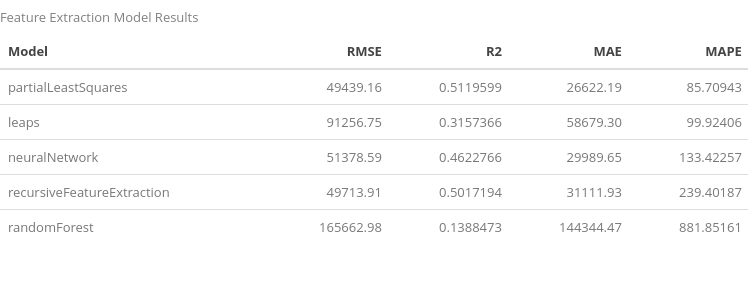
\includegraphics[width=.6\textwidth, height=0.2\textheight]{Images/electricity_psf_fe_summary.png}
\end{subfigure}
\begin{subfigure}{1\textwidth}
\centering
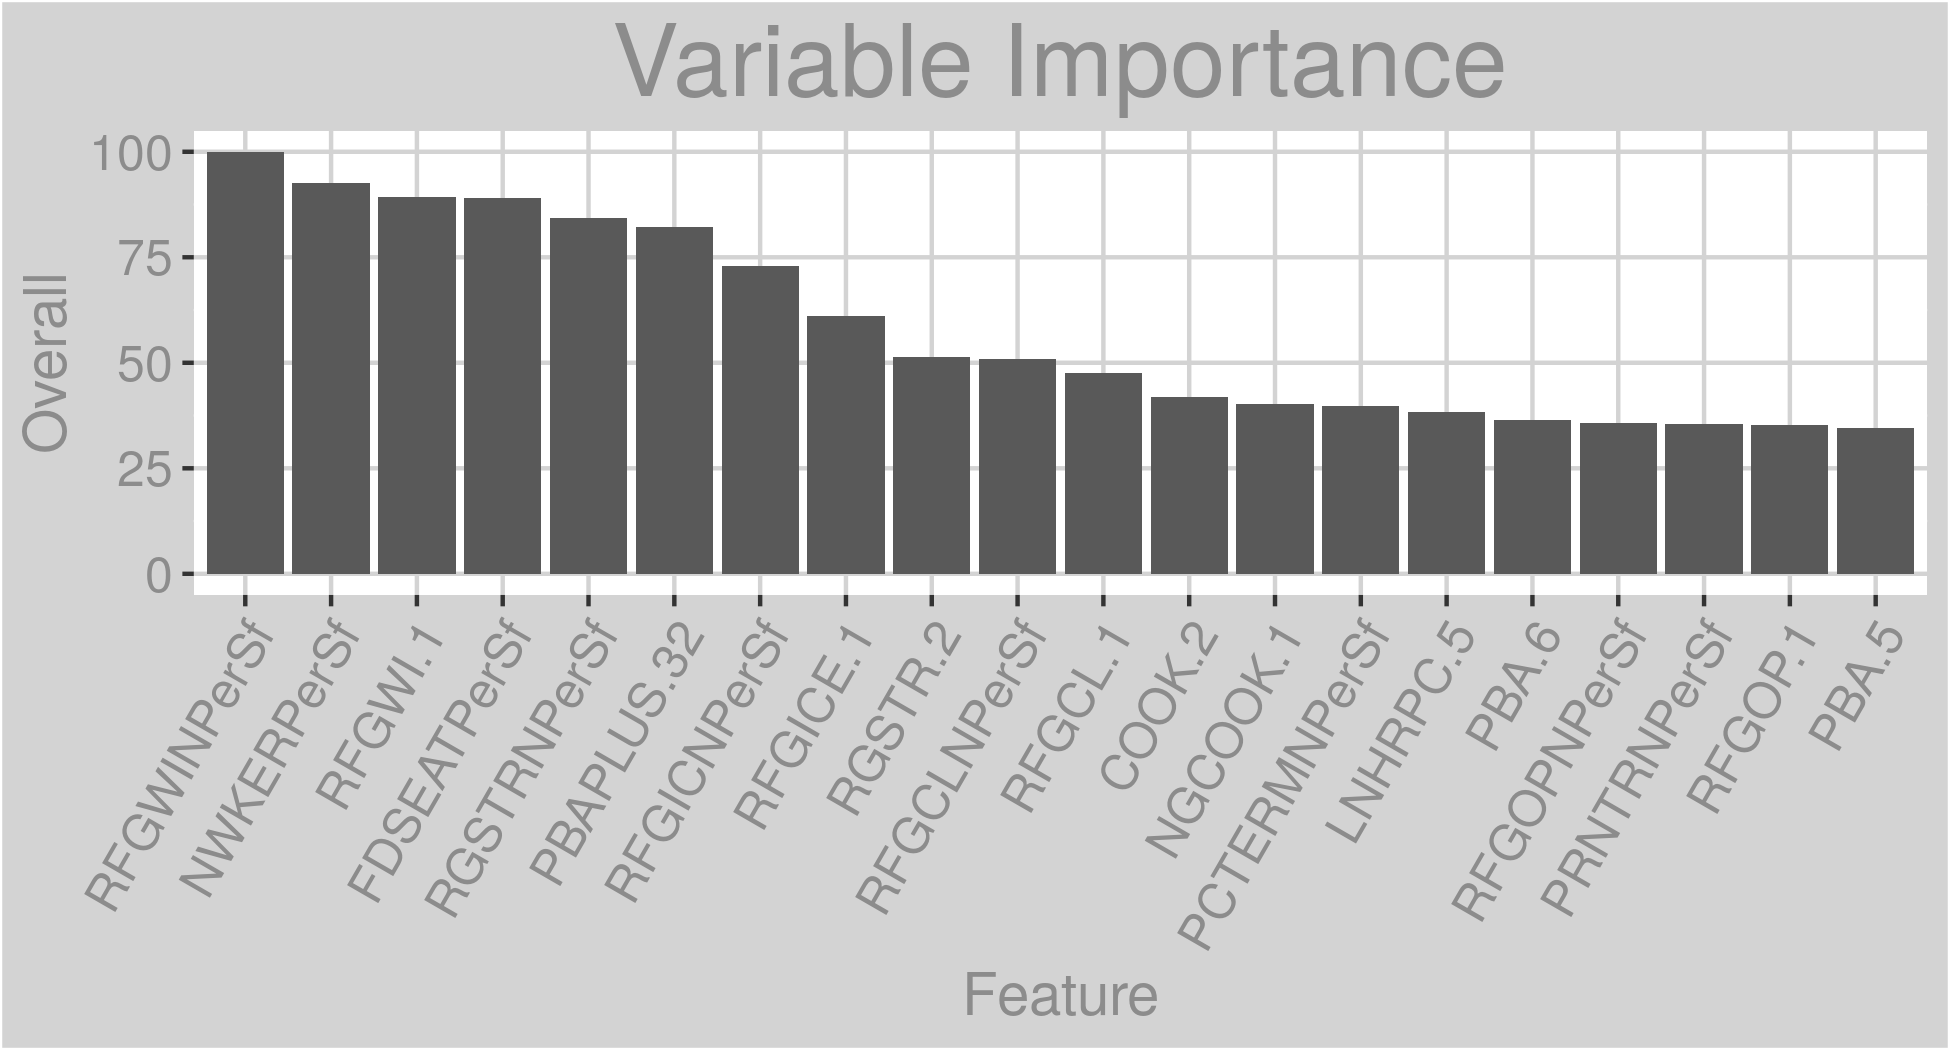
\includegraphics[width=.99\textwidth, height=0.3\textheight]{Images/electricity_psf_all_vars.png}
\end{subfigure}
\end{figure}
In order to rank the most impactful features, the variable importance metrics from the selected models were all set to the same scale then summed up.  As a preliminary check, the top 20 predictors are plotted in the appendix and are generally discussed here.  It seems the attempts to create stratified random samples may have been beneficial in this case since there are some building type specific end-uses that are highly ranked.  As previously noted, there are many attributes associated with refrigeration, office, and food sales equipment.  Also, the attribute identifying one of the more atypical building types, speaking in an energy intensity sense, has made it into the top 20 (\lstinline{PBA.5[NON-REFRIGERATED WAREHOUSE]}).  Additionally, some occupancy features (\lstinline{NWKERPerSf}, \lstinline{FDSEATPerSf}) have been included which is expected given that they impact interior space cooling and ventilation loads. In an attempt to truly follow the imporant predictors, no variables have been removed from this set and the order of importance remains unchanged.  \textit{\hyperref[appendix:electricity:sva]{Appendix}}
%Electricity - Variable selection
%Electricity - Predictor vs. Response analysis
%Electricity - neural netowrk model
%Performance Experiments \\
%Conclusion \\
%Future Work \\
%Acknowledgements \\
%Citations \\
%Appendices \\
\end{document}